\chapter{Implementation of iVector System}

In this chapter we will go over the implementation details of the iVector system. Since we couldn't test the system using the Gaussian backend during development, most implementation decisions in this chapter were decided with the identification rate of classifier on 30 second development iVectors using the max score wins techinque described in section \ref{sect:multiclass}.

\section{Classifier}

To classify iVectors, we used the LIBLINEAR library \footnote{\url{http://www.csie.ntu.edu.tw/~cjlin/liblinear/}}. It is optimized for linear classification on large sets of data and features \cite{liblinear}, well documented and supports both SVM-based or logistic regression classification. We normalized iVectors according to the techniques in section \ref{sect:svmnormal}. Using a standard iVector implementation, we tested both the OVO and OVR approach to multiclass classification. We found a slight adaption of the OVR approach to perform best. When a dialect was the $+1$ class, we didn't use the other dialect of the same language in the $-1$ class. This simpler classification task greatly reduced the identification error rate for the two-dialect languages, while the identification rate for the other languages remained more or less the same. This technique did not extend that easily to OVO classification as dialects would then have less tests than the other languages. The number of wins, or sum of scores for a language would then have to be normalized by the number of classes it was tested against. This more complicated treatment of dialects had little effect on the identification performance which was about the same as we got when using standard OVR. 

We tested three approaches to set the penalty-parameter for the regularized classifier. For all three approaches we tested a finite set of parameters against development vectors. In the first test we assumed that each classifier would use the same penalty-parameter, and simply chose the parameter that got the highest total identification rate. For the other two approaches the penalty-parameter was set independently for each classifier the OVR-bank consisted of. This was performed by either maximizing the number of correctly labeled utterances minus the incorrectly labeled, or maximizing the sum of soft scores for a document belonging to it's true class. Using the same penalty parameter slightly but consistently outperformed the other methods. 

In our identification tests, the SVM and logistic regression gave comparable results. The similar iVector system from \cite{lrivector} still reported that the system performed better on language detection tasks when it used logistic regression. This is perhaps not so unexpected if we use backend score-calibration since the soft-scores from the logistic regression is a more meaningfull interpretation of the class assignment confidence than the distance from decisionboundary-score we get from SVMs. Allthough we didn't get to verify this argument, we decided to logistic regression.

LIBLINEAR also uses the same interface as LIBSVM \footnote{\url{http://www.csie.ntu.edu.tw/~cjlin/libsvm/}} which allowed us easily to experiment with non-linear classifiers as well. For the non-linear SVM we followed the developers of LIBSVM's guide to SVM classification \cite{practicalsvm}. Their recommendations did not yield a classifier that performed better than the linear classifiers regardless of the iVector dimension. We expect that with more experimentation we could have gotten better results with kernel based classifiers. There should be parameters that make some non-linear classifiers behave as if they are linear \cite{keerthi2003asymptotic}. This means that the performance of the linear classifier is a lower bound for the performance we could achieve with a non-linear classifier, but the time required to search for SVM parameters did however take considerably longer for the non-linear classifiers. Since it seemed like the iVectors were just as separable with a linear decision boundary, we did not investigate using non-linear SVMs further. 

\section{Document Vector}
\label{sect:docvectlength}

We use the same process as in \ref{sect:phonetranscription} to generate the phoneme transcripts that are used to construct the document vectors. As expected, the system performed better when no mapping of the phoneme labels were used. Although this result was consistent for all the tests we ran, the savings in computational complexity was significant enough for us to use the mapping for some of our experiments. We used only trigrams as features in the document vector as bigram and unigram counts did not seem to add supplementary information to the vector. In fact the identification rate on 30 second development utterances slightly decreased when we included bigrams and unigrams as features. There was a more significant drop in performance when we used the square root of trigram counts as features. E.g. for a typical iVector-implementation, we experienced more than a $20$ \% relative decrease in the error rate when ordinary features were used. This result contradicts the findings from the similar iVector system given in \cite{lrivector}. A possible reason for this might be that the other system used phoneme lattices which would make the document vectors more rich in information. Without lattices, it might just be harmful to spread the significance of trigrams to those with lower counts.

From the gradient of $\mathbf{T}$ and iVectors given in equations \ref{tgrad} and \ref{ivectgrad} we see that a maxima isn't affected by the number of features in the utterance as long as the direction of the document vector is the same. We trained the total variability matrix using utterances with a length of about five minutes of speech. The reason for not matching the training utterance length with the test utterance length were twofold. It is difficult to exploit the sparsity of the document vectors, so having fewer training utterances with more features reduced the time required to train the system significantly. We also expect that the direction of the document vector will be more influenced by noise when the utterance is short. If the total variability matrix were trained on short vectors, then it would also have to model more of this noise that cannot be used to recognize languages. In a way, we can then view the shorter development and test utterances as projected into the less noisy subspace when we find their iVectors. This frees up dimensions in the iVector to model more important features. We didn't do an extensive search for the optimal training utterance length, but the identification rate was a bit higher when we used 5 minute rather than 4 or 6 minute training utterances.

After training $\mathbf{T}$ with longer utterances, it might have been beneficial to train the classifier with iVectors from shorter utterances. The classifier would then have more training data available, and the training iVectors would come from utterances of more similar lengths to the test data. This turned out to be true for the mapped phonemes document vectors, where the absolute performance increased slightly when the classifier was trained with two miniute long utterances.Without the phoneme mapping, there was no change in the performance, but the classifier ended up with a less regularized model. This might indicate that even though there would be more variance in the short duration iVectors, the decision boundaries between classes weren't much affected. Instead the classifier would more frequently mislabel some of the training vectors. Since shorter training utterances would increase the training time and not provide any significant increase in performance, we opted to use the five minute utterances for training of the classifier as well.


\section{Vanilla iVector system}
\label{sect:vanillaivect}

For the basic iVector system we implemented the techniques described in section \ref{sect:ivecttrain} and \ref{sect:ivectextract}. The total variability matrix is then trained with the iterative approach of one update of the ivectors from the train set using equation \ref{ivectupdate} and one update of the matrix using equation \ref{tupdate}. Pseudocode for the algorithm is given in appendix \ref{ap:vanivecttrain}. We used an iVector dimension of $200$. This is substantially lower than the $600$ dimension iVectors used in \cite{lrivector}, but that system had more training documents, and used phoneme lattices to produce more dense document vectors. The log-likelihood for training and development documents during a typical training can be seen in figure \ref{fig:vanivecttrainlike}. 
\begin{figure}[hbt]
	\begin{center}
	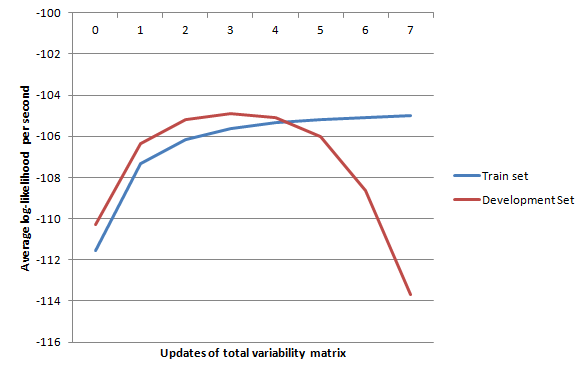
\includegraphics{figures/vanivecttrainlike.png}
	\caption{Average log-likelihood per second of speech for training and development data during the training algorithm after 0 to 7 iterations. The iVector dimension was set to $200$.}
	\label{fig:vanivecttrainlike}
	\end{center}
\end{figure}
In the figure, the devtest documents can have a slightly higher log-likelihood than the training documents. This is because we ignore the features in the development document vectors that aren't seen in the training set since they would have an likelihood of $-\infty$. The development utterances then seem to have fewer features per second of speech. This effect makes it difficult to directly compare the training likelihoods against development likelihoods, but what we do see is the effect of over-fitting the model to the training data when we use too many iterations of the algorithm. For this reason we stop training $\mathbf{T}$ when a decrease in likelihood for development vectors are observed. In figure \ref{vanivecttrainlike} we would observe an decrease in likelihood during the fourth iteration, so the optimal matrix $\mathbf{T}$ would be the one we found in the third iteration. We also implemented the safeguard against making too large update steps described in section \ref{sect:higherlike}, but it had only a minimal effect on the iVectors.

When extracting iVectors either for training the classifier, or testing the performance of the classifier, we initialize the iVectors to zero. We then do a number of iterations of updating equation \ref{ivectupdate} using the total variability matrix we found during training. Since theese are the iVectors that will be used for classification, it seems natural to also take a look at how the iVectors during extraction react to the trained total variability matrix. In figure \ref{fig:vanextractlike} we show the achieved likelihood for the first 6 iterations of the extraction algorithm for total variability matrices trained in 0 to 7 iterations. Figure \ref{fig:vanextractdevlike} confirms what we saw in figure \ref{fig:vanivecttrainlike}, that too many iterations of updating $\mathbf{T}$ will give the model a worse fit to development utterances. This effect of over-fitting is however not so clear in this figure when the documents are given many iterations to find the likelihood maxima. Still the maximum, regardless of the number of iterations during extraction, is reached when the total variability matrix is trained with around three iterations.

\begin{figure}[hbt!]
	\begin{center}
		\subfloat[ ]{
			\label{fig:vanextracttrainlike}
			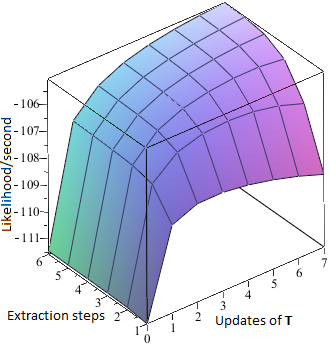
\includegraphics[width=0.5\textwidth]{figures/rottrainlike.png}
		}
		\subfloat[ ]{
			\label{fig:vanextractdevlike}
			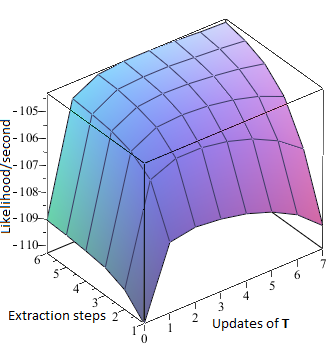
\includegraphics[width=0.5\textwidth]{figures/rotdevlike.png}
		}
	\end{center}
	\caption{Average log-likelihood per second of speech when extracting iVectors with 1 to 6 iterations using a total variability matrix trained in 0 to 7 iterations. (a) likelihood for training documents, (b) development documents. For both tests the iVector dimension was set to 200.}
	\label{fig:vanextractlike}
\end{figure}

Figure \ref{fig:vanextracttrainlike} showing the likelihood for training iVectors is more troublesome. As expected the figure shows that when $\mathbf{T}$ is trained with more iterations, there will exist iVectors that will give the training data higher likelihood. The problem is that when the iVectors are initialized to zero, it may take many iterations of the extraction algorithm before any benefit of a more fitted $\mathbf{T}$-matrix is shown. With only one iteration of extracting iVectors, the likelihood will actually decrease for training data if $\mathbf{T}$ is trained with more than three iterations. While this decrease in likelihood is only present after $\mathbf{T}$ is over-trained for training utterances, the underlying problem might be a cause of concern as it may limit the performance of the system even when $\mathbf{T}$ is trained with fewer iterations. We suspect the problem to be that as $\mathbf{T}$ gets more fitted to specific iVectors, the Hessian, or second derivative, to the log-likelihood will change more rapidly in the iVector space. This can make the updates of iVectors converge slower because the Hessian in a Newton Raphson update is approximated to be constant between the old and new vectors. 

%A notable difference between the likelihoods for training and development utterances, shown in figure \ref{fig:vanextractlike}, is that the development utterances has more potential to improve the likelihood than training utterances when $\mathbf{T}$ is untrained. This is probably because the development utterances are of shorter duration and sparser.

\section{Reset-Trained iVector System}

One possible solution to the problems with the default system would be to train the total variability matrix using the iVectors we would get during the first few iterations of iVector extraction. Instead of perforiming iterations of updating iVectors and then update $\mathbf{T}$, each iteration could be to train iVectors from zero and then update $\mathbf{T}$. For our system we only used one update of the iVectors per iteration. This keeps the computational requirements during training similar to the standard system, while the total variability matrix is optimized to give documents a high likelihood from the first iteration of the iVector extraction process. 

\begin{figure}[hbt!]
	\begin{center}
	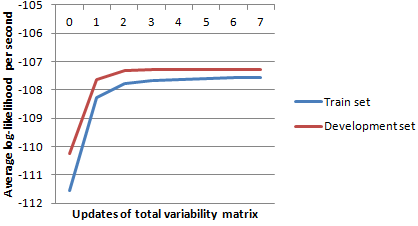
\includegraphics{figures/resetlike.png}
	\caption{Likelihood for training and development utterances during training when iVectors are reset to zero before each iteration. The iVector dimension was 200.}
	\label{fig:resetlike}
	\end{center}
\end{figure}

The likelihoods for training and development documents during this training process is shown in figure \ref{resetlike}. From the figure we see that the likelihood for both training and development utterances ceases to increase after a few iterations and $\mathbf{T}$ never becomes over-fitted to the training data. Still the likelihoods during this training method is smaller than the likelihoods we got using the standard training method, shown in figure \ref{fig:vanivecttrainlike}. This is not so unexpected since we restrict the iVectors by resetting them before each iteration. During iVector extraction, where the iVectors are given more iterations to converge to their maxima, this difference in likelihood vanishes.

\begin{figure}[hbt!]
	\begin{center}
	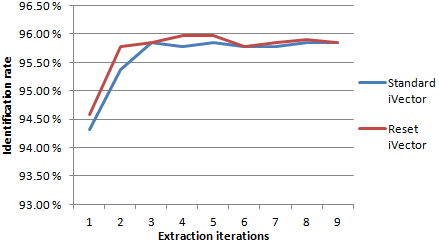
\includegraphics{figures/resetidentification.png}
	\caption{Identificaiton rate for 200-dimensional iVectors. The horizontal axis denotes the number of iterations used during extraction to produce the iVectors for training and testing the system}
	\label{fig:resetidrate}
	\end{center}
\end{figure}

In figure \ref{fig:resetidrate} we compare the identification rate of the standard and reset-trained sytems on 30 second development vectors. As expected the reset-trained system has a higher identification rate when iVectors are extracted with few iterations. It is more surprising that the identification rate for the standard system doesn't exceed the reset trained system at any iteration. We're not sure of the reason for this, or if this improvement extends to other data-sets. It might be that the reset-training results in less \emph{model variance}, since $\mathbf{T}$ is trained on iVectors that have only captured coarse details of the utterances. 

\section{iVector Dimension}
\label{sect:ivectdimtests}

A very important parameter that hasn't been much discussed is the iVector dimension. Since there will be more degrees of freedom, it seems natural that a higher iVector-dimension will result in lower likelihood for both training and development vectors. Still, this does not mean that we should use iVectors of high dimension. A high likelihood does not neccessarily mean that the system will perform better, and using low-dimension iVectors is less computational intensive.  In figure \ref{fig:dimidrate} we show the identification rate for the standard and reset-trained iVector system. We have both trained and tested the classifier using iVectors that where extracted with the same number of Newton Raphson updates. This follows our previous logic of accommodating so that training, development and test iVectors all come from as similar as possible statistical distributions. The number of iterations that gave the best result varied with each system. As we see, the reset-trained system consistently outperformed the regular system regardless of dimension. Most notably, it performed much better at lower dimensions.

\begin{figure}[hbt!]
	\begin{center}
	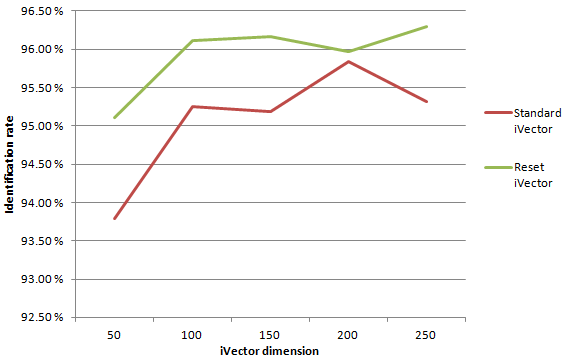
\includegraphics{figures/dimidentification.png}
	\caption{Identification rate for standard and reset-trained iVector system with different dimensions. The rates were measured from 30 second development utterances.}
	\label{fig:dimidrate}
	\end{center}
\end{figure}

It should be noted that the difference between the best and the worst results is only about 35 more correctly identified utterances out of about 1500. We only try a discrete set of penalty-parameters for the classifier, and also plain luck might simply make a few utterances in an iVector-space of some dimension barely cross over the decision boundary to the wrong or correct class. This explains some of the noise in the performance results, and why it is difficult to see clear trends in the performance when increasing or decreasing the performance. The dimension that performed best in the test might not objectively be best suited to separate the languages, and it is no guarantee that it will perform best on the NIST test set. For the final system we used the $150$-dimensional reset-trained iVector system. Although the $250$ dimensional system performed slightly better on the devtest vectors, the high dimensionality made the system much slower to train and test. The $150$-dimensional system performed best when iVectors where extracted with four iterations of Newton Raphson updates.

\section{System for Shorter Duration Utterances}

In the past sections we have based our design decisions for the iVector systems performance on 30 second utterances. At least to some degree, many of these decisions should be valid for the 10 and 3 second tests as well. In section \ref{sect:docvectlength} we argued that the total variability matrix could, and should, be trained using long-duration utterances. For the reset-trained total variability matrix, over-fitting wasn't an issue, so it would probably make little difference for the final matrix to check for over-fitting using shorter duration development vectors. This all suggests that the same total variability matrix could be used for utterances of all sizes. 

We are however not sure that the same iVector dimension will be optimal for utterances of all lengths. Shorter utterances will have sparser document vectors, and perhaps reduce the need for high-dimensional iVectors. This was not checked, and we used the $150$-dimensional reset-trained total variability matrix for 10 and 3 second utterances as well. In section \ref{sect:docvectlength} we found no significant improvement when training the classifier with shorter utterances than what we used when training the total variability matrix. It is possible that there would be clearer performance benefits of using shorter utterances to train the classifiers for 10 and 3 second utterances. The number of utterances will increase if each utterance is shorter, and extracting 3 or even 10 second training utterances for the classifier using the whole training set would simply take too long. A possible solution would be to train the classifier with short utterances from only a subset of the training set, but this was not tested. Since we expect the system to have a worse performance on shorter utterances, the development utterances had the same length as the test utterances.  This allows us to optimize the classifiers penalty-parameter for each test. 
















%Strain 92.6732673267 - 4min
%Ltrain 92.6732673267 - rett under 5 min
%new200 92.9372937294 - 6min
%new200 94.9834983498
%bigram 92.1452145215

%nomap nolimit 95.7755775578
%nomap            94.5214521452

%twosetord 93.33333333